\documentclass[conference]{IEEEtran}
\usepackage{cite}
% \usepackage{amsmath,amssymb,amsfonts}
\usepackage{amsmath}% equation formatting
% \usepackage{algorithmic}% Algorithms
\usepackage{graphicx}
\graphicspath{{img/}}
% \usepackage{textcomp}% Text Companion fonts
\usepackage[usenames,dvipsnames]{xcolor}
\def\BibTeX{{\rm B\kern-.05em{\sc i\kern-.025em b}\kern-.08em
    T\kern-.1667em\lower.7ex\hbox{E}\kern-.125emX}}

\usepackage[cmintegrals]{newtxmath}% equation font similar to the rest
\usepackage{microtype}
\usepackage[T1]{fontenc} %set the font (output) encoding
% \usepackage[brazil]{babel} %"sumário", "capítulo", etc.
\usepackage{hyphenat}
% \hyphenation{mate-mática recu-perar}
\usepackage{cite}
\usepackage{booktabs}
\usepackage{listings}
\makeatletter
\let\@ORGmakecaption\@makecaption
\long\def\@makecaption#1#2{\@ORGmakecaption{#1}{#2}\vskip\belowcaptionskip\relax}
\makeatother
\lstdefinestyle{mystyle}{
frame               = single,
rulecolor           = \color{gray},
basicstyle          = \ttfamily\scriptsize,
belowcaptionskip    = 8pt,
aboveskip           = 8pt,
belowskip           = 8pt,
columns             = fullflexible,
breakatwhitespace   = false,
breaklines          = true,
keepspaces          = true,
showspaces          = false,
showstringspaces    = false,
inputencoding       = utf8,
extendedchars       = true,
literate            =
{á}{{\'a}}1 {é}{{\'e}}1 {í}{{\'i}}1 {ó}{{\'o}}1 {ú}{{\'u}}1
{Á}{{\'A}}1 {É}{{\'E}}1 {Í}{{\'I}}1 {Ó}{{\'O}}1 {Ú}{{\'U}}1
{à}{{\`a}}1 {è}{{\`e}}1 {ì}{{\`i}}1 {ò}{{\`o}}1 {ù}{{\`u}}1
{À}{{\`A}}1 {È}{{\'E}}1 {Ì}{{\`I}}1 {Ò}{{\`O}}1 {Ù}{{\`U}}1
{ä}{{\"a}}1 {ë}{{\"e}}1 {ï}{{\"i}}1 {ö}{{\"o}}1 {ü}{{\"u}}1
{Ä}{{\"A}}1 {Ë}{{\"E}}1 {Ï}{{\"I}}1 {Ö}{{\"O}}1 {Ü}{{\"U}}1
{â}{{\^a}}1 {ê}{{\^e}}1 {î}{{\^i}}1 {ô}{{\^o}}1 {û}{{\^u}}1
{Â}{{\^A}}1 {Ê}{{\^E}}1 {Î}{{\^I}}1 {Ô}{{\^O}}1 {Û}{{\^U}}1
{œ}{{\oe}}1 {Œ}{{\OE}}1 {æ}{{\ae}}1 {Æ}{{\AE}}1 {ß}{{\ss}}1
{ç}{{\c c}}1 {Ç}{{\c C}}1 {ø}{{\o}}1 {å}{{\r a}}1 {Å}{{\r A}}1
{€}{{\EUR}}1 {£}{{\pounds}}1 {ã}{{\~a}}1 {Ã}{{\~A}}1,
showtabs=false,
tabsize=2,
}
\lstset{}
\lstset{style=mystyle}

\usepackage{xurl}

% \renewcommand{\figureautorefname}{Fig.}%
% \renewcommand{\tableautorefname}{Tabela}%
% \renewcommand{\equationautorefname}{Equação}%
% \renewcommand{\lstlistingname}{Listagem}%

\usepackage{placeins}% \FloatBarrier
\usepackage[bottom]{footmisc}% \footnote
%\setlength{\skip\footins}{.5cm}

\usepackage{lipsum}

% Warning: multiple PDFs with page group incluided in a single page
\pdfsuppresswarningpagegroup=1

% Mandatory to load hyperref as the last package
\usepackage[colorlinks,urlcolor=blue]{hyperref}

%----------------------------------------
% user defined commands
%----------------------------------------
\newcommand{\F}[1]{\footnote{\url{#1}}}

% Last edited: 2023-12-02

%========================================
\begin{document}
%========================================

\title{Data-Driven Parameter Discovery of a One-Dimensional Burgers' Equation Using a Physics-Informed Neural Network}

\author{
	\IEEEauthorblockN{1\textsuperscript{st} Eduardo F. Miranda}
	\IEEEauthorblockA{\textit{Applied Computing (CAP)} \\
	\textit{National Institute for Space Research} \\
	São José dos Campos, Brazil \\
	efurlanm@gmail.com}
	\and
	\IEEEauthorblockN{2\textsuperscript{nd} Leonardo B. L. Santos}
	\IEEEauthorblockA{\textit{Applied Computing (CAP)} \\
	\textit{National Institute for Space Research} \\
	São José dos Campos, Brazil \\
	santoslbl@gmail.com }
	\and
	\IEEEauthorblockN{3\textsuperscript{rd} Stephan Stephany}
	\IEEEauthorblockA{\textit{Applied Computing (CAP)} \\
	\textit{National Institute for Space Research} \\
	São José dos Campos, Brazil \\
	stephan.stephany@inpe.br}
}

\maketitle
\thispagestyle{plain}  % set page numbering
\pagestyle{plain}

\begin{abstract}
This work demonstrates the use of a Physics-Informed Neural Network (PINN) trained to solve supervised learning tasks respecting the law of physics described by the one-dimensional Burgers partial differential equation (PDE), and focuses on the problem of data-driven PDE parameter discovery. The Burgers' equation is one PDE with derivatives in space and time that is commonly solved by a numerical method. However, recent work proposes the use of PINN to solve, as a new class of data-efficient universal function approximators, which naturally encode any underlying physical laws as prior information. As the number of sample points required for efficient Deep Natural Network (DNN) training would be very high, PINN was proposed, allowing the use of a smaller number of sample points, and incorporating the related physical equation in the simulation. This work evaluates the discovery of parameters of the Burgers' equation through the use of PINN, for different hyperparameters and dataset sizes, seeking the best adjustment. The relative errors and processing times obtained are presented, running on the LNCC's Santos Dumont supercomputer.
\end{abstract}

% \begin{IEEEkeywords}
% component, formatting, style, styling, insert
% \end{IEEEkeywords}

%----------------------------------------
\section{Introduction}
%----------------------------------------

Many simulations are mathematically modeled by Partial Differential Equations (PDEs), which have derivatives in space and time. However, the coefficients of these derivatives are unknowns, and the PDEs are usually solved by a numerical method, like the finite difference method. Recent works proposed to solve PDEs using Deep Neural Networks (DNN), which are machine learning algorithms. The universal approximation theorem states that a neural network can approximate any continuous function, as long as the network has a sufficient number of hidden layers and employs nonlinear activation functions.
This approach requires knowledge of a large set of sample points in space and time domain (called Collocation Points - CPs) to train the DNN, which can be obtained either by observation, or if the model is known, it can be generated by numerical methods. 
As the required number of CPs would be very high, Physics-Informed Neural Networks (PINNs) were proposed and allow the use of a smaller number of CPs as they include the underlying physical laws related to the simulation in the DNN.   


PINNs can be used in direct problems (inference or solution), where the PDE and parameters are known and we want to obtain the simulation result, and in inverse problems (identification or discovery) where we have the dataset and want to obtain the PDE parameters.
A work by Chevallier et al. \cite{Chevallier2000} describes a speedup of 7 using DNN to obtain parameters in the Longwave Radiative Transfer model from ECMWF (European Center for Medium-Range Weather Forecasts), showing the importance of using DNN to obtain parametric representation in numerical modeling of various atmospheric processes.
Krasnopolsky et al. \cite{Krasnopolsky2006} also cites speedups between $10$ to $10^5$ using DNN in the parametrization of physical models in oceanic and atmospheric numerical models.
Furthermore, there is also the possibility of using PINN in cases where the model (or the PDE that describes it) is known, to reduce the size of the dataset necessary to train the DNN, thus increasing efficiency, or in cases where there is noise in the sample and we want the underlying physical law to help deal with it.

This work evaluates data-driven parameter discovery of the one-dimensional Burgers' equation, a PDE with derivatives in space and time, obtained through PINN, for different hyperparameters and dataset sizes.
The work seeks to answer the question “what is the ideal combination of hyperparameters and dataset size, for this specific problem?”, in order to seek the best model for the expected result.

The PINN discovery is evaluated in terms of accuracy and DNN training processing time, executed on the Santos Dumont supercomputer (SDumont) at the National Scientific Computing Laboratory (LNCC). The tests were carried out on a Bull Sequana X1120 processing node with two 2.1 GHz 24-core Intel Xeon Gold 6252 Skylake processors (totaling 48 cores), 384 GB of main RAM, and four Nvidia Volta V100 GPUs. Only one GPU is used in this work. All data and codes used in this manuscript are publicly available on GitHub at \url{https://github.com/efurlanm/425/}.

The discovery of EDPs by PINNs is relatively recent and the acquisition of knowledge in this approach can be useful for application in some specific modules of numerical models used at CPTEC/INPE for weather and climate prediction. 

%----------------------------------------
\section{Material and methods}\label{sec:meth}
%----------------------------------------

Raissi et al. \cite{Raissi2019} published an article about PINNs, which has 7217 citations (December 2023). That work defines PINNs as DNNs trained to solve supervised learning tasks, but complying to physical laws, usually described by nonlinear PDEs. It also describes the use of DNNs to solve PDEs and obtain physics-informed surrogates of the physical model that are fully differentiable in all coordinates and free parameters. PINNs form a new class of data-efficient universal function approximators, which can be effectively trained using small datasets, and which may encode any underlying physical law. 

DNN training data can be randomly sampled from observational data, or through simulations using synthetic data from a numerical model. Except for synthetically generated data, as long as a sufficient number of CPs are available, a standard DNN can solve the PDE, otherwise a PINN would be required. A PINN uses a specific loss function incorporating PDE and parameters, in such a way that during the training phase using the set of CPs, the applicable physical law is incorporated \cite{Cuomo2022}.

PINNs can be considered neural networks for supervised learning problems, as proposed here. However, PINNs can also be used as agents for Reinforcement Learning (RL) \cite{Cuomo2022}. The most common PINN architectures are Multi-layer Perceptrons (MLPs), Convolutional Neural Networks (CNNs) and Recurrent Neural Networks (RNNs). Newer architectures are Auto-Encoder (AE), Deep Belief Network (DBN), Generative Adversarial Network (GAN) and Bayesian Deep Learning (BDL) \cite{Cuomo2022}. This work uses the MLP architecture.

The proposed test problem requires the parameters discovery of a particular one-dimensional Burgers' equation, which estimates the speed field $u$ along time (\autoref {eq:burg}). Training data for the PINN is given by a set of CPs corresponding to the position field in different times are randomly generated within the considered domain.
 
In the train phase, the neural network then estimates a solution $u(t,x)$.
The function employed by the PINN, $f(t,x)$ (\autoref {eq:ftx}), is derived from the known Burgers' equation, and allows to calculate the loss function.
The parameters of the differential operator that we want to obtain are transformed into PINN parameters.
In the following equations, the differential operator parameter $\lambda_1$ (or $u$) is the speed of fluid at the indicated spatial and temporal coordinates, the differential operator parameter $\lambda_2$ (or $\nu$) is the kinematic viscosity of fluid, and the subscripts denote partial differentiation in time and space, respectively, as
$u_t$ (which denotes $\frac{du}{dt}$), 
$u_x$ (which denotes $\frac{du}{dx}$), and 
$u_{xx}$ (which denotes $\frac{d^2u}{dx^2}$).

\begin{flalign}\label{eq:burg}
	u_t + \lambda_1 u_x - \lambda_2 u_{xx} = 0, \quad x \in [-1,1], \ t \in [0, 1]
\end{flalign}

The Burgers' equation is employed to evaluate the error $f$ of the solution $u(t,x)$ estimated by the PINN, as shown in \autoref {eq:ftx}.

\begin{equation}\label{eq:ftx}
	f := u_t + \lambda_1 u_x - \lambda_2 u_{xx}
\end{equation}

In this work, the PINN loss function to be minimized is given by the mean squared error (\autoref {eq:mse}) of two components, $MSE_u$, which embeds the training data on $u(t,x)$, and $MSE_f$, which embeds the structure imposed by \autoref{eq:burg}, where $t$ is the time step, and $x$ is the one-dimension coordinate. The neural network parameters, along with the differential operator parameters $\lambda_1$ and $\lambda_2$, can be learned by minimizing the MSE.

\begin{equation}\label{eq:mse}
	MSE = MSE_u + MSE_f
\end{equation}
where
$$ MSE_u = \frac{1}{N}\sum_{i=1}^{N}|u(t^i_u, x^i_u)-u^i|^2 $$
and
$$ MSE_f = \frac{1}{N}\sum_{i=1}^{N}|f(t^i_u, x^i_u)|^2 $$

The $\{t^i_u, x^i_u, u^i\}^N_{i=1}$ denotes the training data on $u(t, x)$, the $MSE_u$ loss corresponds to the training data in $u(t, x)$, and the $MSE_f$ loss imposes the structure of \autoref{eq:burg} on a finite set of CPs. The number and location of CPs are the same as the training data.

In this work a dataset of 2,000 points generated by the numerical Gaussian Quadrature Method (GQM), using $ \lambda_1 = 1 $ and $ \lambda_2 = 0.01/\pi $, was used to obtain the CPs, that are also used to compare the result obtained through PINN. The GQM method is an iterative numerical algorithm that approximates the definite integral of a function as a weighted sum of the function values at specified points within the domain of integration \cite{Burkardt2013}.

When training a PINN, some important adjustable hyperparameters are the number of hidden layers $N_l(l = 1, 2, ...)$, and the number of neurons in each layer $N_{le}(e = 1, 2, ...)$. A general understanding about $N_l$ and $N_{le}$ is that efficient adjustment is still an unsolved problem and the determination is made empirically \cite{Xu2022}.

The results obtained in this work using DNN are subject to the problem of overfitting and underfitting. Overfitting means that the DNN performs very well when using training data, but fails as soon as it needs to deal with new data in the problem domain, that is, it does not generalize. Underfitting, on the other hand, means that the model performs poorly on both datasets, i.e., it does not fill the model. Both issues can also negatively affect performance \cite{Koehrsen2018}.

The Relative L2 Error used in this work is introduced here as defined in \autoref{eq:error} where $ \| \widehat{U} - U \| $ is the L2 norm of the prediction deviation at certain time, and $\|U\|$ denotes the L2 norm of the synthetic data at that time. $R_{L2}$ gives good quantification of the prediction accuracy at a certain time \cite{Xu2022}.

\begin{equation}\label{eq:error}
R_{L2} = \frac{\| \widehat{U} - U \|}{\|U\|}
\end{equation}

% ----------------------------------------
\subsection{PINN Implementation}
% ----------------------------------------

The specific PINN architecture implemented in this work is an MLP network with an input layer of 2 neurons, a number of hidden layers ranging from 1 to 8, with each hidden layer having a number of neurons ranging from 10 to 30, and a output layer with one neuron. The loss function is the mean squared error (MSE). Minimization of the loss function is performed by an optimization method, the generalized limited-memory Broyden-Fletcher-Goldfarb-Shanno (L-BFGS) algorithm, a quasi-Newton method. All hidden layers employ the hyperbolic tangent as the activation function. The implementation has been configured to stop training when it reaches 50,000 iterations or when the hardware's floating point precision is interfering with the calculated error.

The PINN implementation is based on the work of Raissi et al. (2019) \cite{Raissi2019} and uses the TensorFlow\F{http://www.tensorflow.org} 1.15 library and the Python 3.7 interpreter. Code snippets of the TensorFlow library are shown in \autoref {lst:utx} and \autoref {lst:ftx}. The code was run on SDumont and uses a V100 GPU. 

\begin{lstlisting}[language=Python, label=lst:utx, caption={Code snippet that implements $u(t,x)$}]
def neural_net(self, X, weights, biases):
	num_layers = len(weights) + 1
	H = 2.0 * (X - self.lb) / (self.ub - self.lb) - 1.0
	for l in range(0, num_layers - 2):
		W = weights[l]
		b = biases[l]
		H = tf.tanh(tf.add(tf.matmul(H, W), b))
	W = weights[-1]
	b = biases[-1]
	Y = tf.add(tf.matmul(H, W), b)
	return Y

def net_u(self, x, t):
	u = self.neural_net(tf.concat([x, t], 1), self.weights, self.biases)
	return u
\end{lstlisting}

\begin{lstlisting}[language=Python, label=lst:ftx, caption={Code snippet that implements $f(t,x)$}]
def net_f(self, x, t):
	lambda_1 = self.lambda_1
	lambda_2 = tf.exp(self.lambda_2)
	u = self.net_u(x, t)
	u_t = tf.gradients(u, t)[0]
	u_x = tf.gradients(u, x)[0]
	u_xx = tf.gradients(u_x, x)[0]
	f = u_t + lambda_1 * u * u_x - lambda_2 * u_xx
	return f
\end{lstlisting}

To obtain the results, first the network is trained until the parameters are obtained, then the prediction is made and compared with the values of the training dataset, which is used both to train the network and compare the results. The implementation does not clearly divide the dataset into training, validation, and testing, however it would be an improvement to be investigated in future work.

%----------------------------------------
\section{Results}\label{sec:resu}
%----------------------------------------

The following results are divided into 4 parts, in the last 3 the number of neurons per layer is fixed on the horizontal axis, and the vertical axis varies according to the number of layers and size of the dataset. In the first part the result is shown in the form of a graph rendered as a pseudo-colored image showing $t$, $x$ and $u(t,x)$ (visual evaluation of the PINN's predictive accuracy), and also a slice at time $t=0.5$. In the second part, the vertical axis is the number of layers (“Neurons x Layers” for simplicity), and in the third part it is the size of the dataset (“Neurons x Dataset” for simplicity). The fourth and final part shows the prediction time for some number of neurons per hidden layer and number of layers. The size of the dataset in some cases is called CP, meaning the same thing.

%----------------------------------------
\subsection{Visual assessment}
%----------------------------------------

A visual assessment of PINN's predictive accuracy is shown in \autoref{fig:bur1}, with time $t$ on the horizontal axis and spatial coordinate $x$ on the vertical axis. The color scale refers to the speed $u(x,t)$. The black marks on the graph represent 2,000 CPs randomly generated and used for training, and to obtain them $ \lambda_1 = 1 $ and $ \lambda_2 = 0.01/\pi $ were used. The network architecture used is composed of 4 hidden layers with 20 neurons each. The white solid vertical line at $t=0.5$ represents a specific snapshot shown in \autoref {fig:bur2}, which shows the overlapping solutions for PINN and GQM. For this specific result, the equation obtained by PINN is $u_t + 0.99958 u_x - 0.0032199 u_{xx} = 0$ whereas the equation used to obtain the training dataset is $u_t + u_x - 0.0031831 u_{xx} = 0$ . The network is able to identify the underlying partial differential equation with remarkable accuracy.

\begin{figure}[htb]\
\centering
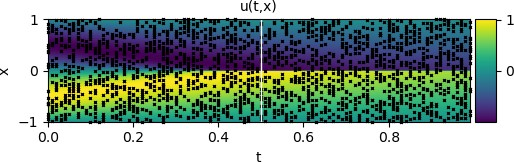
\includegraphics[width=\linewidth]{burg-01.jpg}
\caption{Predicted solution u(t, x) along with the training data. The horizontal axis denotes time $t$, and the vertical axis, the coordinate $x$. The marks in the graph represent the randomly assigned CPs used for training. The color scale refers to the speed u(t, x). The solid white vertical line refers to the snapshot $t=0.5$ shown in \autoref{fig:bur2}.} 
\label{fig:bur1}
\end{figure}

\begin{figure}[htb]
\centering
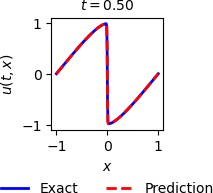
\includegraphics[width=.4\linewidth]{burg-02.jpg}
\caption{Superimposed solutions for PINN (in red) and numerical solution (in blue) for the $t=0.5$ snapshot.}
\label{fig:bur2}
\end{figure}

%----------------------------------------
\subsection{Neurons x Layers}
%----------------------------------------

For the results presented below, the hyperparameters $N_{l}$ (number of hidden layers) and $N_{le}$ (number of neurons per hidden layer) were varied, as well as the number of CPs for training.
The \autoref{tab:resu1} shows the relative L2 errors and training times of the neural network, for different hyperparameters used: 10, 15, 20, 25, and 30 neurons per hidden layer, and 1, 2, 4, 6, and 8 hidden layers.
The number of CPs was set at 2,000.
All values shown here are the average of 3 runs.
In this table it is possible to observe that there is a tendency for the best values to be concentrated in the center, probably because there is a problem of underfitting or overfitting in the values at the edges of the table. One of the highlights is that the smallest error is obtained with 6 hidden layers, not 8. In this specific case, increasing the number of layers not only does not increase precision, but also worsens performance.

\begin{table}[htb]
\centering
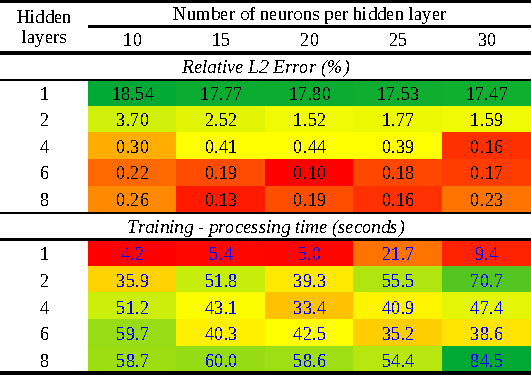
\includegraphics[width=.95\linewidth]{rlayerror2.pdf}
\caption{Relative L2 errors and DNN training times for different number of neurons and hidden layers. On the color scale, the best values are highlighted in red.}
\label{tab:resu1}
\end{table}

The \autoref{fig:rlaygrapherror2} shows that the error for 1 hidden layer is high compared to the other number of layers. For 2 layers there is a significant improvement in accuracy. For 4, 6, and 8 the gain in precision is not that great, but the curves are similar and are in the region of greater precision, showing that they would be the best choices.

\begin{figure}[htb]
	\centering
	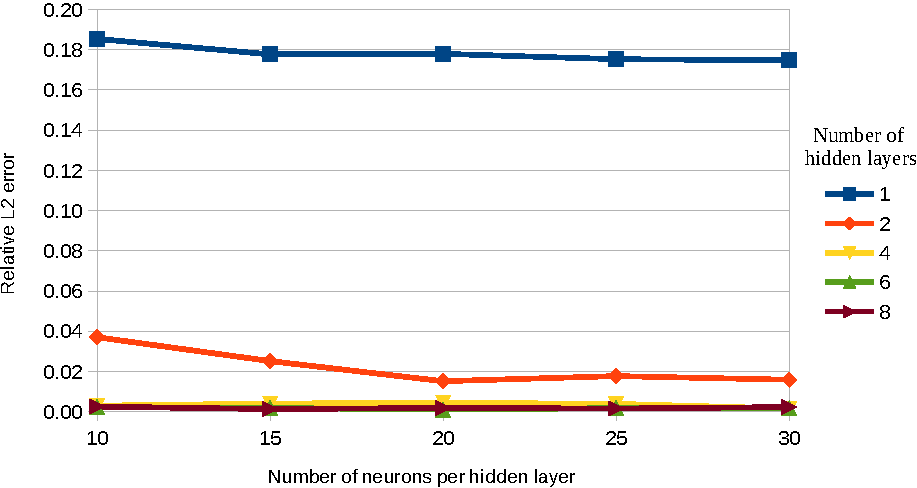
\includegraphics[width=\linewidth]{rlaygrapherror2}
	\caption{Relative L2 error (\%) in function of number of neurons and hidden layers.}
	\label{fig:rlaygrapherror2}
\end{figure}

The \autoref{fig:rlaygraptime2} shows for 4 hidden layers, a tendency to describe a curve that resembles a parabolic, with a minimum processing time of 20 neurons per hidden layer. This is probably due to the problem of underfitting and overfitting occurring at the beginning and at the end of the curve.

\begin{figure}[htb]
	\centering
	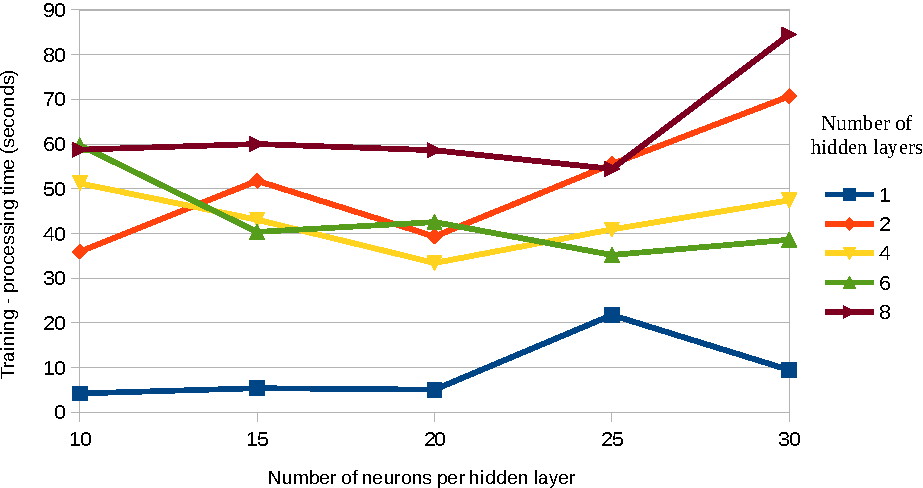
\includegraphics[width=\linewidth]{rlaygraphtime2}
	\caption{Processing times (seconds) in function of number of neurons and hidden layers.}
	\label{fig:rlaygraptime2}
\end{figure}

%----------------------------------------
\subsection{Neurons x Dataset}
%----------------------------------------

The table \autoref{tab:rnu8error2} shows the relative L2 errors and training times of the neural network, for different hyperparameters and number of CPs used: 10, 15, 20, 25, and 30 neurons per hidden layer, and 400, 800, 1200, 1600, and 2000 CPs.
The number of layers was set at 8.
All values shown here are the average of 3 runs.
In this table, as in the previous one, it is possible to observe that there is a tendency for the best values to be concentrated in the center, probably because the problem of underfitting or overfitting is occurring in the values at the edges of the table. One of the highlights is that considering the smallest error and the shortest processing time, the best dataset size is 1600, and the best number of neurons per hidden layer is 20.

\begin{table}[htb]
	\centering
	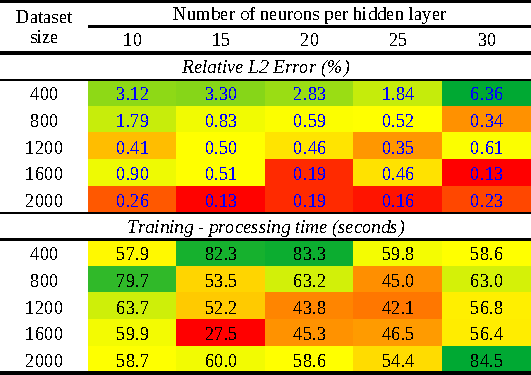
\includegraphics[width=.95\linewidth]{rnu8error2.pdf}
	\caption{Relative L2 errors and DNN training times for different number of neurons and dataset size. The number of hidden layers is set to 8. On the color scale, the best values are highlighted in red.}
	\label{tab:rnu8error2}
\end{table}

The \autoref{fig:rnu8grapherror2} shows that the error for 400 CPs is high compared to the others, 800 CPs presents a significant improvement in precision, and the other curves are relatively close, not presenting such a large accuracy gain.

\begin{figure}[htb]
	\centering
	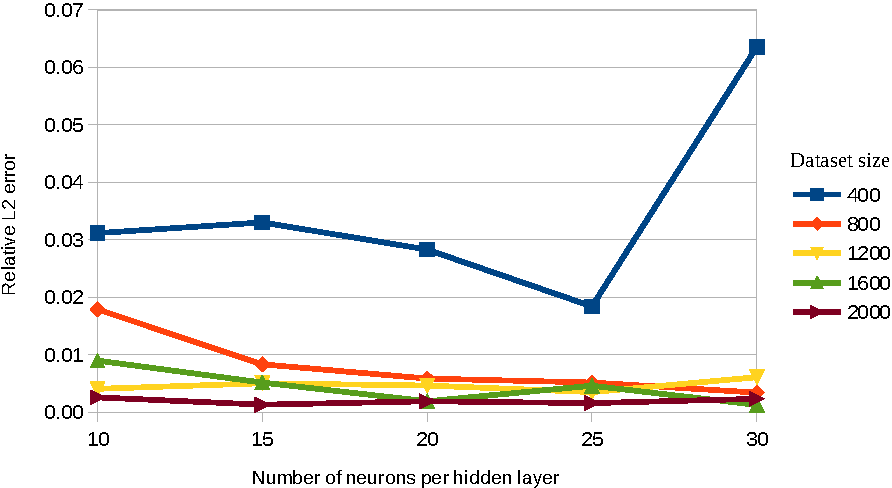
\includegraphics[width=\linewidth]{rnu8grapherror2.pdf}
	\caption{Relative L2 error (\%) in function of number of neurons and dataset size. The number of hidden layers is set to 8.}
	\label{fig:rnu8grapherror2}
\end{figure}

The \autoref{fig:rnu8graphtime2} shows for most curves a tendency to describe a curve that resembles a parabolic, probably due to the problem of underfitting and overfitting occurring at the beginning and end of the curve. The shortest processing time occurs for 15 neurons per hidden layer, and 1600 CPs.

\begin{figure}[htb]
	\centering
	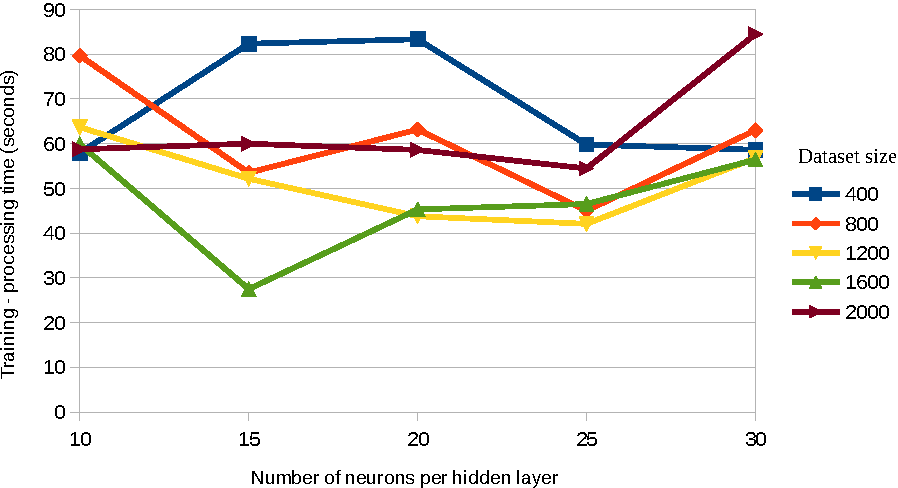
\includegraphics[width=\linewidth]{rnu8graphtime2.pdf}
	\caption{Processing times (seconds) in function of number of neurons and dataset size. The number of hidden layers is set to 8.}
	\label{fig:rnu8graphtime2}
\end{figure}

%----------------------------------------
\subsection{Prediction time}
%----------------------------------------

The \autoref{tab:rpre} shows the neural network's prediction times, once training is complete. Times are for 10, 20, and 30 neurons per hidden layer, and 1, 4, and 8 layers. Most times are relatively close, around 0.7 seconds. Compared to the training time of about 43 seconds in the best cases, the time to predict the final result represents about 1.5\% of the training time, relatively. The difference is very large, and shows that we should look for algorithms or solutions where the number of trainings is smaller than the number of predictions, when  applicable.

\begin{table}[htb]
	\centering
	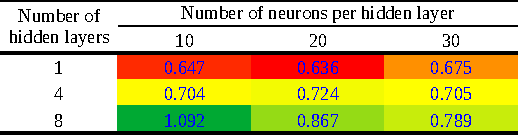
\includegraphics[width=.95\linewidth]{rpre2.pdf}
	\caption{Prediction times for different number of neurons and hidden layers. On the color scale, the best values are highlighted in red.}
	\label{tab:rpre}
\end{table}

%----------------------------------------
\section{Conclusions}\label{sec:conc}
%----------------------------------------

This work evaluates data-driven parameter discovery for a one-dimensional Burgers' equation using a Physics-Informed Neural Network (PINN). The Burgers' equation is a fundamental partial differential equation (PDE) with derivatives in space and time, which is commonly solved by a numerical method. An evaluation of the relative error and required training time, performed in SDumont, is also presented for different hyperparameters and dataset sizes. It was possible to observe that adjusting the hyperparameters and the size of the dataset is important for obtaining performance when using PINN. The implementation also proved to be relatively simple, and the results easy to obtain. As deep learning technology continues to grow rapidly, both in terms of methodological and algorithmic developments, this could be a timely contribution that can benefit a wide range of scientific domains.
As future work, it would be interesting to explore other PINN architectures, as well as taking advantage of the parallel use of GPU.

%----------------------------------------
\section*{Acknowledgment}
%----------------------------------------

Authors thank LNCC (National Laboratory for Scientific Computing) for grant 205341 AMPEMI (call 2020-I), which allows access to the Santos Dumont supercomputer (node of the SINAPAD, the Brazilian HPC system).



% The asterisk symbol (*) is used to indicate that a environment does not produce numbering
%----------------------------------------
% \section*{References}  % Keep commented
%----------------------------------------

\FloatBarrier
\bibliographystyle{IEEEtran}
\bibliography{library}

%========================================
\end{document}
%========================================





